\documentclass[\main.tex]{subfiles}

\chapter{Metodologia de Operacionalização do Trabalho}

\section{Processo e Metodologia de Trabalho}
Foi adotada uma abordagem iterativa incremental, com algumas reuniões de acompanhamento ao
longo do projeto. No decorrer de 15 semanas, foram criadas 4 iterações pelas quais foram
divididas as tarefas em cima descritas.\par
O \textit{\gls{roadmap}} do projeto, que se encontra representado na forma de um diagrama de
Gantt, apresenta, mais detalhadamente, a atribuição das tarefas nas diferentes iterações e a
duração das mesmas.
\vspace{5pt}

\begin{figure}[h]
\centering
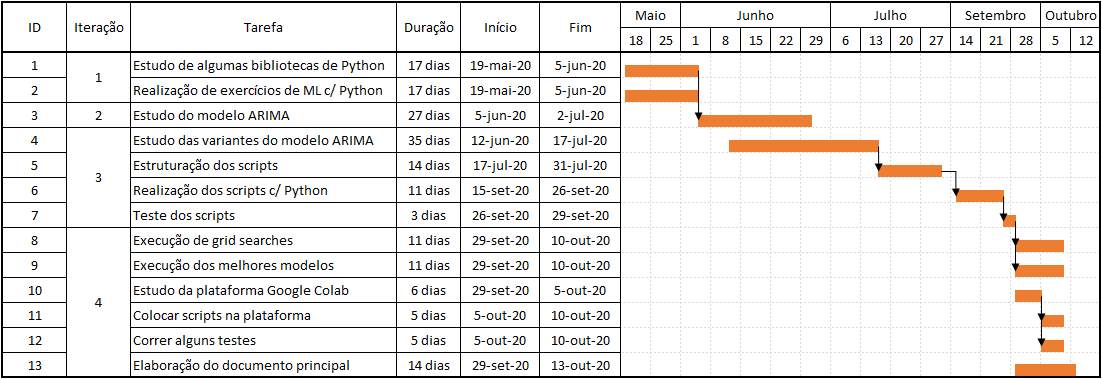
\includegraphics[width=\linewidth]{../private_assets/Roadmap.png}
\caption{Diagrama de Gantt representativo do \textit{\gls{roadmap}} do projeto}
\end{figure}


\newpage
\section{Arquitetura Concetual}
A arquitetura do projeto (representada na figura 4.2) garante três componentes principais: o
conversor de \textit{\glspl{dataset}} procura no diretório de \textit{\glspl{dataset}},
dentro do sistem de ficheiros, e transforma o conjunto de dados selecionado num objeto
\textit{\say{DataFrame}} da biblioteca \textit{pandas}; o otimizador de modelos permite
testar um ou mais modelos com o \textit{\gls{dataset}} carregado anteriormente; o exportador
de resultados e registos arquiva o sumários dos resultados (tempo de execução,
\textit{\acrshort{mae}}, \textit{\acrshort{mse}}, \textit{\acrshort{rmse}}) e os registos
(mensagens de sucesso ou de erro) para todos os modelos testados na mesma sessão. Todo este
ambiente pode ser implementado no \textit{\gls{google colab}}.\par

\begin{figure}[h!]
\centering
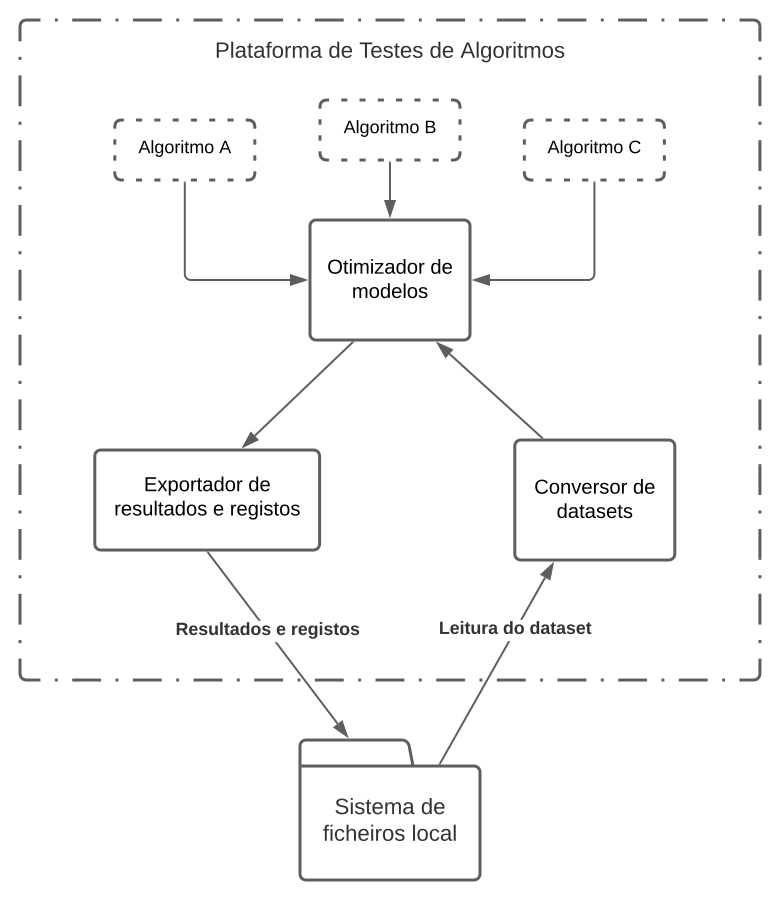
\includegraphics[width=0.8\linewidth]{../private_assets/Arquitetura_App.png}
\caption{Arquitetura da aplicação}
\end{figure}\par

Na \acrfull{poo}, o encapsulamento refere-se ao agrupamento de dados com os métodos que
operam nesses dados ou à restrição do acesso direto a alguns dos componentes de um objeto.
\cite{encapsulation_paul_rogers} O encapsulamento é utilizado para ocultar os valores ou o
estado de um objeto de dados estruturados dentro de uma classe, evitando o acesso direto de
terceiros não autorizados a eles.\par
Este mecanismo não é exclusivo para \acrshort{poo}. Implementação de dados abstratos, como
por exemplo módulos, oferecem uma forma semelhante de encapsulamento. A similaridade foi
explicada por teóricos da linguagem de programação em termos de tipos existenciais.
\cite{data_abstraction_existentials}\par
Para a realização deste projeto foi necessário a utilização de encapsulamento, de modo a
manter uma boa estrutura e organização do código.\par
Em relação à estrura das pesquisas em grelha, foram todas desenhadas e pensadas à medida do
projeto, a fim de testar o maior número possível de modelos para um determinado
\textit{\gls{dataset}}.\par


\section{Desenvolvimento da Solução}
O desenvolvimento dos algoritmos está representado no diagrama de classes presente na
figura 4.3.

\begin{figure}[h!]
\centering
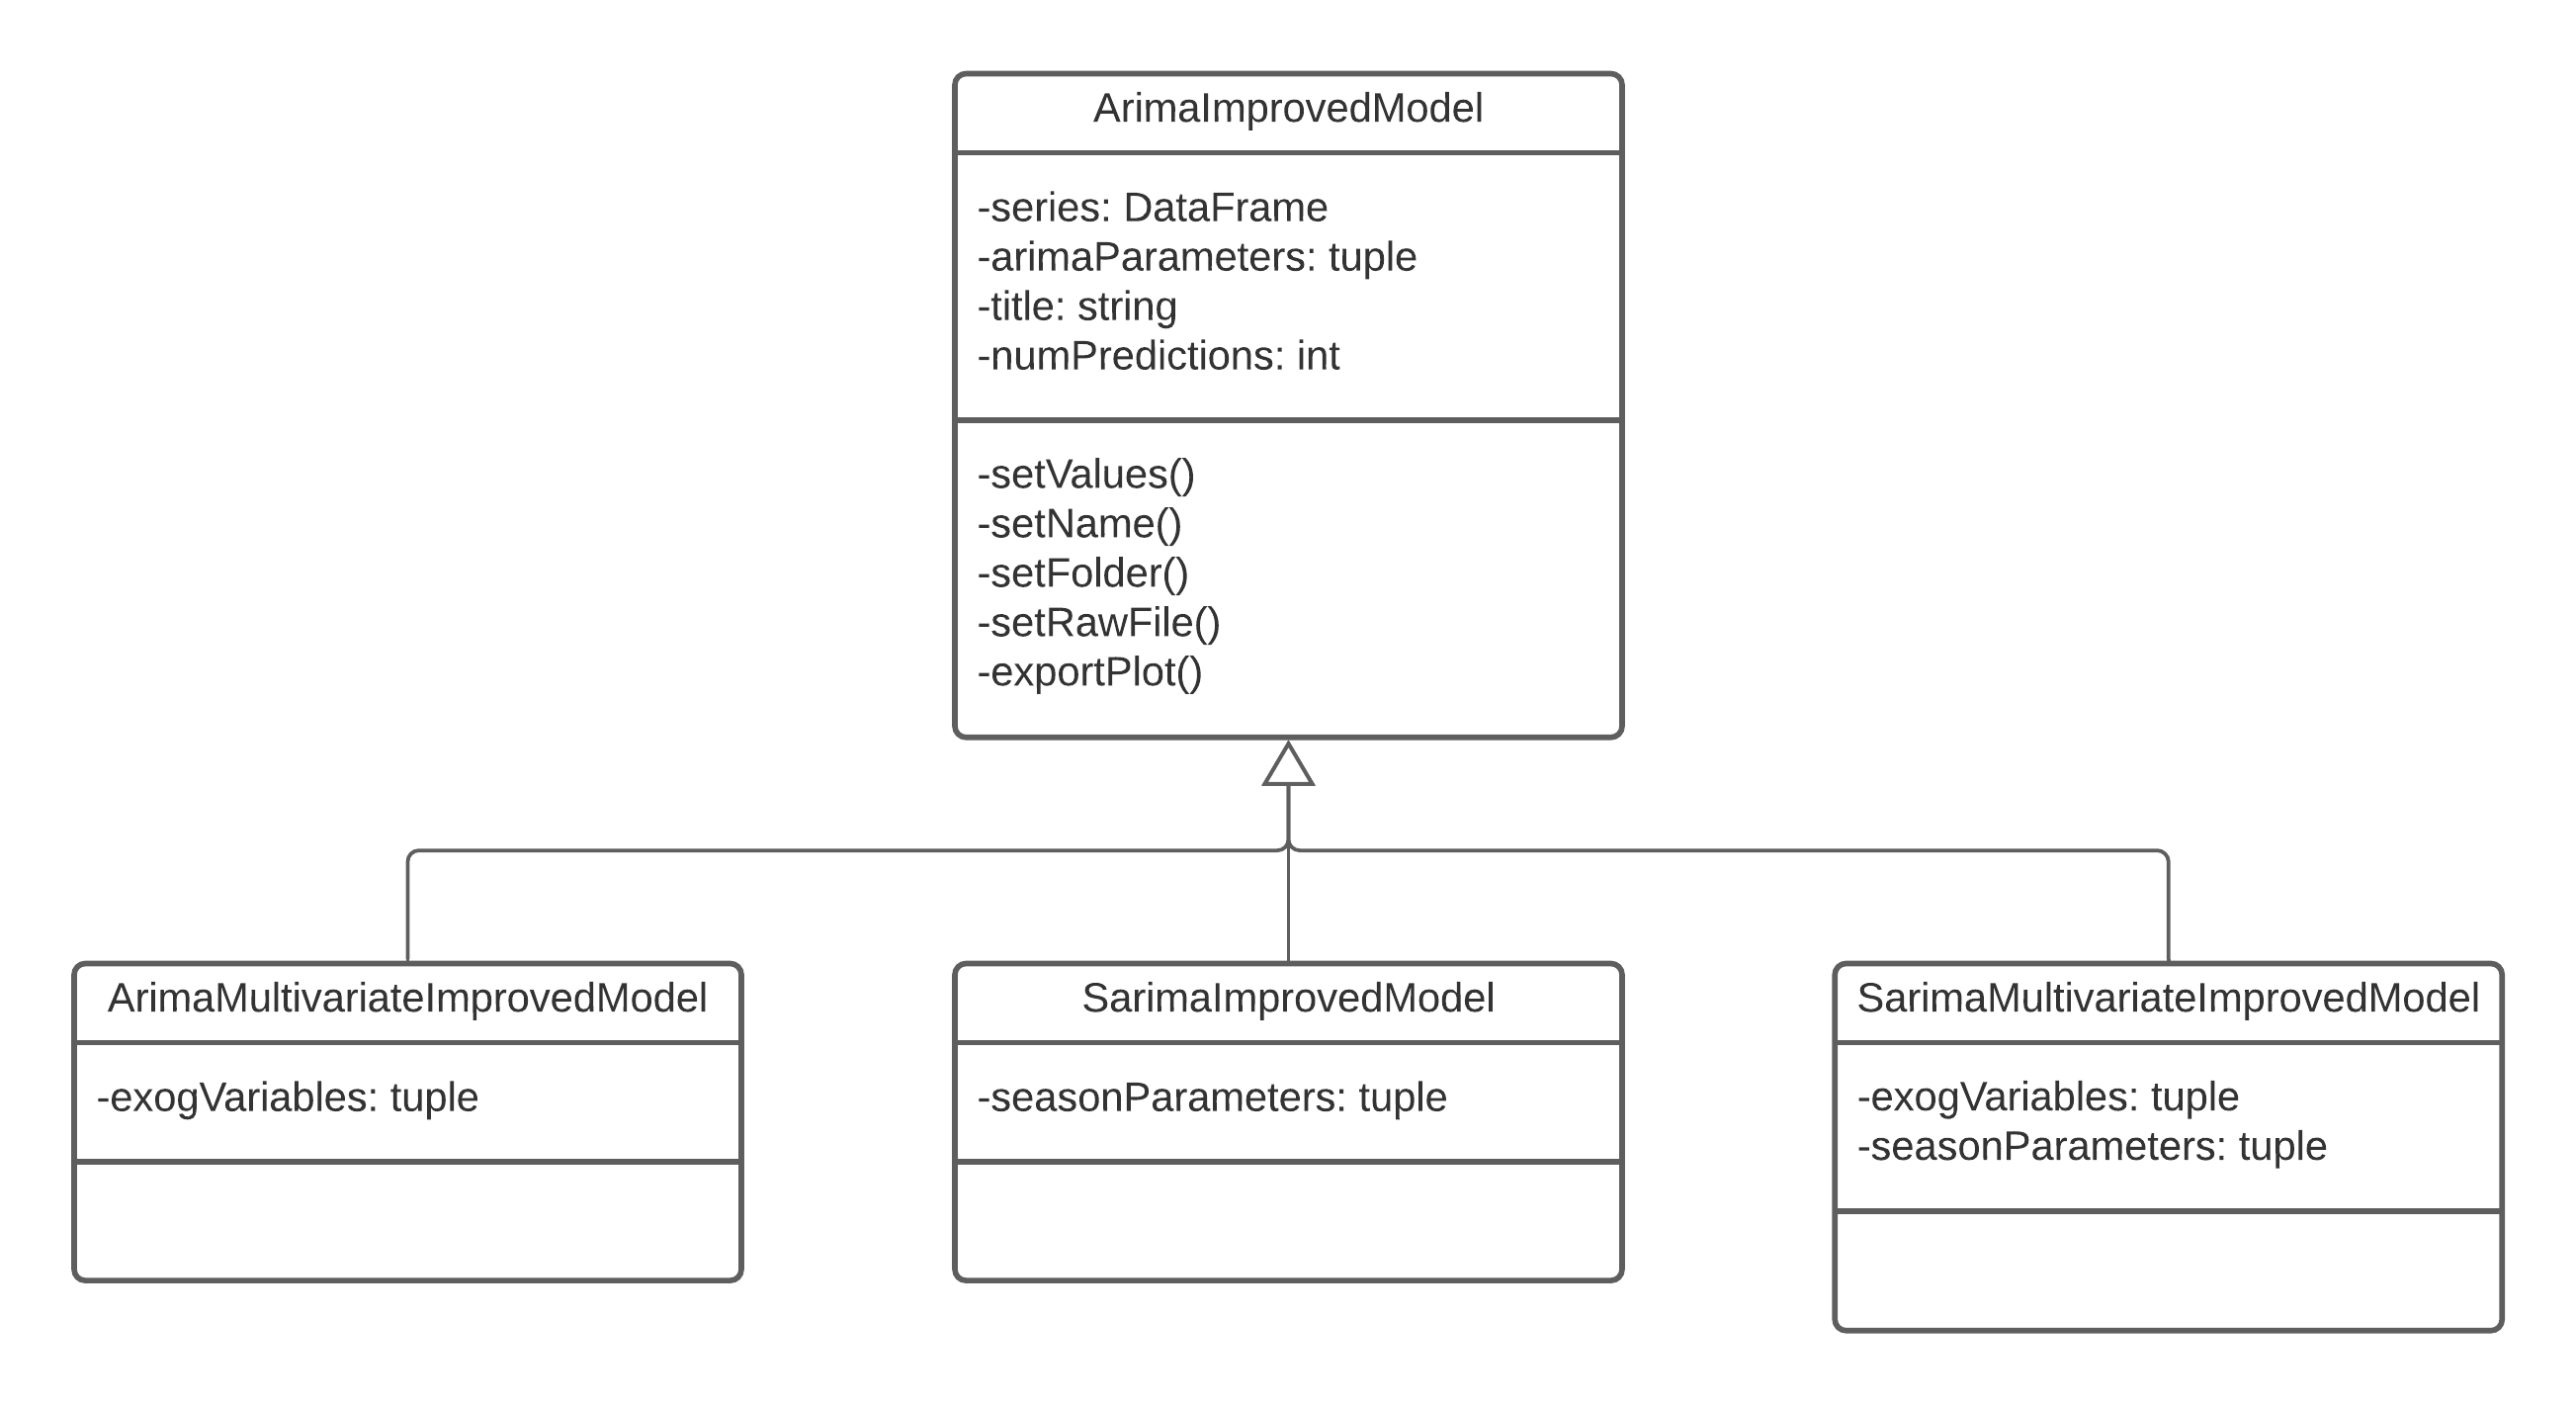
\includegraphics[width=\linewidth]{../private_assets/ClassDiagram_App.png}
\caption{Diagrama de classes dos algoritmos implementados}
\end{figure}\par


\subsection{Modelo Genérico}
Em primeiro lugar, o \textit{GenericModel} trata-se de um modelo genérico, como o próprio
nome indica. Esta classe tem como objetivo ser uma \gls{classe abstrata}, isto é, não deve
ser instanciada, serve apenas para servir de modelo para outras classes. Neste caso em
específico, como a linguagem utilizada é \textit{\gls{python}} não existe nenhuma
nomenclatura especial para este tipo de dados. Está representada no excerto de código 4.1.

\newpage
\begin{lstlisting}[language=Python, caption=Classe do modelo genérico]
    class GenericModel:
    """Class that represents the structure of the Generic Model for the creation
    of specific models


    Author: Luis Marques
    """

    MODEL_NAME: str = "GENERIC"

    def __init__(self, series: DataFrame,
                 variable_to_predict: str,
                 arima_parameters: tuple,
                 title: str = "",
                 num_splits: int = 0,
                 num_predictions: int = 10,
                 predictions_size: float = 0.0):
        """Creates an instance of an GenericModel.

        Args:
            series (DataFrame): series of the dataset to run the model.
            variable_to_predict (str): name of the variable to predict. It must
                be the same name of the column in the dataset.
            arima_parameters (tuple): parameters of the arima model.
            title (str): title of the model. Used to differentiate this model
                from other ones with the same parameters. Defaults to "".
            num_splits (int): number of splits to do in the dataset. Defaults
                to 0.
            num_predictions (int): number of predictions of the model. Defaults
                to 10. It will only have effect if the predictions_size is equal
                to zero.
            predictions_size (float): percentage of data to predict (from 0 to
                1). Defaults to 0.
        """

        self.series = series
        self.variable_to_predict = variable_to_predict
        self.arima_parameters = arima_parameters
        self.title = title
        if predictions_size == 0.0:
            self.num_predictions = num_predictions
        else:
            self.num_predictions = int(len(self.values) * predictions_size)
        self.data_split = 0
        self._set_values()
        self.predictions = list()
        if num_splits == 0:
            self.train = self.values[:-self.num_predictions]
            self.test = self.values[-self.num_predictions:]
            self.history = [x for x in self.train]
            self._set_name()
            self._set_folder()
            self._set_raw_file()
            self._execute()
        else:
            for train_index, test_index in TimeSeriesSplit(n_splits=num_splits).split(self.values):
                self.train = self.values[train_index].copy()
                self.test = self.values[test_index].copy()
                self.train = [*self.train, *self.test[:-self.num_predictions]]
                self.test = self.test[-self.num_predictions:]
                self.data_split += 1
                self.history = [x.copy() for x in self.train]
                self._set_name()
                self._set_folder()
                self._set_raw_file()
                self._execute()

    def _execute(self):
        """Executes the model. This method should be implemented in each
        individual model class"""
        pass

    def _set_exog_values(self):
        """Sets the values arrays to be used based on the series and the
        variable to predict. Also sets the exog values to be used in the
        predictions."""
        if hasattr(self, "exog_variables"):
            self.exog_values = self.series.filter(items=self.exog_variables)
            self.exog_values = self.exog_values.values

    def _set_values(self):
        """Sets the values to be used based on the series and the variable to
        predict"""
        self._set_exog_values()
        self.scaler = MinMaxScaler()
        self.values = self.series[[self.variable_to_predict]]
        self.values[[self.variable_to_predict]] = self.scaler.fit_transform(self.values[[self.variable_to_predict]])
        self.values = getattr(self.values, self.variable_to_predict).values

    def _set_name(self):
        """Sets the name of the model according to its variables"""
        self.name = ""
        self.title = "".join(self.title.split())
        if self.title != "":
            self.name += f"{self.title}_"
        self.name += f"{self.MODEL_NAME}("
        for parameter in self.arima_parameters:
            self.name += f"{str(parameter)},"
        if hasattr(self, "season_parameters"):
            self.name = self.name[:-1] + ")("
            for parameter in self.season_parameters:
                self.name += f"{str(parameter)},"
        self.name = self.name[:-1] + ")_"
        self.name += f"predictions_{str(self.num_predictions)}"
        if self.data_split != 0:
            self.name += f"_crossvalidation_{self.data_split}"

    def _set_folder(self):
        """Creates an output folder for the model"""
        self.folder = os.path.join(OUTPUT_FOLDER, self.name)
        try:
            os.makedirs(self.folder)
        except FileNotFoundError:
            shutil.rmtree(self.folder)
            os.makedirs(self.folder)

    def _set_raw_file(self):
        """Creates a raw .csv file to write the predictions of the model"""
        file_name = f"raw_{self.name}.csv"
        file_path = os.path.join(self.folder, file_name)
        self.file = CSVWriter(file_path, ("Predict", self.variable_to_predict))

    def _export_plot(self):
        """Exports the plot of the model"""
        timesteps = numpy.arange(self.num_predictions)

        real_values = ([x for x in self.test])

        prediction_values = ([x for x in self.predictions])

        pyplot.plot(timesteps,
                    real_values,
                    color="green",
                    marker="^",
                    label="Real values")

        pyplot.plot(timesteps,
                    prediction_values,
                    color="red",
                    marker="X",
                    label="Predictions")

        pyplot.ylabel(self.variable_to_predict)
        pyplot.xlabel("Timesteps")
        pyplot.xticks(numpy.arange(min(timesteps), max(timesteps) + 1, 1.0))
        pyplot.grid(which="major", alpha=0.5)
        pyplot.gcf().canvas.set_window_title(self.name)
        pyplot.gcf().set_size_inches(8, 5)
        pyplot.savefig(os.path.join(self.folder, f"plot_{self.name}.png"),
                       format="png", dpi=300)
        pyplot.close()
\end{lstlisting}\par

\newpage
Os parâmetros do método construtor deste modelo genérico são os seguintes:
\begin{itemize}
    \item \textit{series} - série temporal para testar o modelo;
    \item \textit{variable\_to\_predict} - nome da variável do \textit{\gls{dataset}} a prever;
    \item \textit{title} - título do modelo, utilizado para diferenciar o modelo dos restantes.
    Tem como valor por defeito uma \textit{\gls{string}};
    \item \textit{num\_splits} - número de divisões a realizar no conjunto de dados antes de
    realizar os testes. Este parâmetro é utilizado caso seja necessário fazer uma
    \gls{validacao cruzada}. Tem zero como valor por defeito;
    \item \textit{num\_predictions} - número de previsões a realizar. Este parâmetro apenas será
    válido se não for definido nenhuma percentagem do \textit{\gls{dataset}} para testes. Tem
    zero como valor por defeito;
    \item \textit{predictions\_size} - percentagem do \textit{\gls{dataset}} para testes. Se este
    parâmetro for diferente de zero, o \textit{\say{num\_predictions}} não terá efeito. Tem zero
    como valor por defeito.
\end{itemize}\par

Em relação aos métodos, esta classe é constituída pelos seguintes:
\begin{itemize}
    \item \textit{\_execute(self)} - este método deve ser implementado por cada classe que extenda
    a classe do modelo genérico;
    \item \textit{\_set\_exog\_values(self)} - define uma lista de valores das variáveis exógenas;
    \item \textit{\_set\_values(self)} - define uma lista de valores da variável com que vão ser
    realizadas as previsões;
    \item \textit{\_set\_name(self)} - define o nome do modelo, tendo em conta o seu título e as
    configurações;
    \item \textit{\_set\_folder(self)} - cria um diretório para o exportar o gráfico e as previsões
    do modelo;
    \item \textit{\_set\_raw\_file(self)} - cria um ficheiro \textit{.csv} para escrever as previsões
    do modelo;
    \item \textit{\_export\_plot(self)} - exporta o gráfico do modelo.
\end{itemize}\par

Na linguagem \textit{\gls{python}} não existe nenhuma palavra chave para declarar tipos de dados
privados, existe apenas uma convenção que, geralmente, é respeitada. Esta convenção define que,
de modo a declarar tipos de dados privados, deve ser colocado um \textit{underscore} antes de
definir a variável ou método a utilizar. Posto isto, todos os métodos da classe genérica estão
\say{declarados} privados, pois não devem ser chamados fora da classe, isto é, eles são invocados
no momento da instanciação de um novo modelo.\par

\newpage
\subsection{Classe \textit{ARIMA}}
O modelo \textit{\gls{arima}} está representado no código através da classe
\textit{ArimaImprovedModel}, demonstrada no excerto de código 4.2. Esta classe extende a classe
do modelo genérico e apenas é necessário implementar o método de execução dos testes.\par
\vspace{10pt}

\begin{lstlisting}[language=Python, caption=Classe do modelo \textit{ARIMA}]
class ArimaImprovedModel(GenericModel):
    """Class that represents the structure of an ARIMA improved model

    Author: Luis Marques
    """

    MODEL_NAME: str = "ARIMA"

    def __init__(self, series: DataFrame,
                 variable_to_predict: str,
                 arima_parameters: tuple,
                 title: str = "",
                 num_splits: int = 0,
                 num_predictions: int = 10,
                 predictions_size: float = 0.0):
        """Creates an instance of an ArimaImprovedModel.

        Args:
            series (DataFrame): series of the dataset to run the model.
            variable_to_predict (str): name of the variable to predict. It must
                be the same name of the column in the dataset.
            arima_parameters (tuple): parameters of the arima model.
            title (str): title of the model. Used to differentiate this model
                from other ones with the same parameters. Defaults to "".
            num_splits (int): number of splits to do in the dataset. Defaults
                to 0.
            num_predictions (int): number of predictions of the model. Defaults
                to 10. It will only have effect if the predictions_size is equal
                to zero.
            predictions_size (float): percentage of data to predict (from 0 to
                1). Defaults to 0.
        """
        super().__init__(series, variable_to_predict, arima_parameters, title,
                         num_splits, num_predictions, predictions_size)

    def _execute(self):
        """Executes the model"""
        self.starting_time = time.time()
        try:
            predictions = list()
            for timestep in range(self.num_predictions):
                model = ARIMA(self.history, order=self.arima_parameters)
                model_fit = model.fit(disp=0)
                output = model_fit.forecast()
                prediction = output[0][0]
                predictions.append(prediction)
                obs = self.test[timestep]
                self.history.append(obs)

            self.predictions = self.scaler.inverse_transform([predictions])[0]
            self.test = self.scaler.inverse_transform([self.test])[0]

            for timestep in range(self.num_predictions):
                self.file.write_line((str(self.predictions[timestep]),
                                      str(self.test[timestep])))

            self._export_plot()

        except Exception as err:
            logs.append(f"LOG: Model {self.name} exported with an error! {type(err).__name__}: {err}")
            self.execution_time = -1
            self.mae = -1
            self.mse = -1
            self.rmse = -1
            # If it returns an error the model folder is removed
            self.file.close()
            shutil.rmtree(self.folder)

        else:
            logs.append(f"LOG: Model {self.name} exported with success.")
            self.execution_time = time.time() - self.starting_time
            self.mae = mean_absolute_error(self.test, self.predictions)
            self.mse = mean_squared_error(self.test, self.predictions)
            self.rmse = sqrt(self.mse)
            self.file.close()

        finally:
            results.append((f'"{self.name}"', str(self.execution_time),
                            str(self.mae), str(self.mse), str(self.rmse)))
            print(f"Model {self.name} finished.")
\end{lstlisting}\par

Nesta classe não existe nenhum parâmetro adicional, para além dos já definidos no modelo genérico.
Quanto aos métodos, apenas o método \textit{\say{\_execute(self)}} foi implementado para realizar
as previsões de acordo com o algoritmo \textit{\acrshort{arima}}.

\newpage
\subsection{Classe \textit{ARIMAX}}
O modelo \textit{\gls{arimax}} está representado no código através da classe
\textit{ArimaMultivariateImprovedModel}, demonstrada no excerto de código 4.3. Esta classe
extende a classe do modelo genérico e apenas é necessário implementar o método de execução
dos testes.\par
\vspace{10pt}

\begin{lstlisting}[language=Python, caption=Classe do modelo \textit{ARIMAX}]
class ArimaMultivariateImprovedModel(GenericModel):
    """Class that represents the structure of an ARIMAX improved model

    Author: Luis Marques
    """

    MODEL_NAME = "ARIMAX"

    def __init__(self, series: DataFrame,
                 variable_to_predict: str,
                 exog_variables: tuple,
                 arima_parameters: tuple,
                 title: str = "",
                 num_splits: int = 0,
                 num_predictions: int = 10,
                 predictions_size: float = 0.0):
        """Creates an instance of an ArimaMultivariateImprovedModel.

        Args:
            series (DataFrame): series of the dataset to run the model.
            variable_to_predict (str): name of the variable to predict. It must
                be the same name of the column in the dataset.
            exog_variables (tuple): tuple of exogenous variables to help the
                model to predict the values.
            arima_parameters (tuple): parameters of the arima model.
            title (str): title of the model. Used to differentiate this model
                from other ones with the same parameters. Defaults to "".
            num_splits (int): number of splits to do in the dataset. Defaults
                to 0.
            num_predictions (int): number of predictions of the model. Defaults
                to 10. It will only have effect if the predictions_size is equal
                to zero.
            predictions_size (float): percentage of data to predict (from 0 to
                1). Defaults to 0.
        """
        self.exog_variables = exog_variables
        super().__init__(series, variable_to_predict, arima_parameters, title,
                         num_splits, num_predictions, predictions_size)

    def _execute(self):
        """Executes the model"""
        self.starting_time = time.time()
        try:
            predictions = list()
            history_extra = [x.copy() for x in self.exog_values[:len(self.history)]]
            for timestep in range(self.num_predictions):
                test_extra = tuple(self.exog_values[-self.num_predictions + timestep])
                model = ARIMA(self.history, order=self.arima_parameters,
                              exog=history_extra)
                model_fit = model.fit(disp=0)
                output = model_fit.forecast(exog=test_extra)
                prediction = output[0][0]
                predictions.append(prediction)
                obs = self.test[timestep]
                self.history.append(obs)
                history_extra.append(obs)

            self.predictions = self.scaler.inverse_transform([predictions])[0]
            self.test = self.scaler.inverse_transform([self.test])[0]

            for timestep in range(self.num_predictions):
                self.file.write_line((str(self.predictions[timestep]),
                                      str(self.test[timestep])))

            self._export_plot()

        except Exception as err:
            logs.append(f"LOG: Model {self.name} exported with an error! {type(err).__name__}: {err}")
            self.execution_time = -1
            self.mae = -1
            self.mse = -1
            self.rmse = -1
            self.file.close()
            # If it returns an error the model folder is removed
            shutil.rmtree(self.folder)

        else:
            logs.append(f"LOG: Model {self.name} exported with success.")
            self.execution_time = time.time() - self.starting_time
            self.mae = mean_absolute_error(self.test, self.predictions)
            self.mse = mean_squared_error(self.test, self.predictions)
            self.rmse = sqrt(self.mse)
            self.file.close()

        finally:
            results.append((f'"{self.name}"', str(self.execution_time),
                            str(self.mae), str(self.mse), str(self.rmse)))
            print(f"Model {self.name} finished.")
\end{lstlisting}\par

Esta classe, para além dos parâmetros já definidos no modelo genérico, ainda conta com o parâmetro
\textit{\say{exog\_variables}} que representa as variáveis exógenas utilizadas para realizar as
previsões. Quanto aos métodos, apenas o método \textit{\say{\_execute(self)}} foi implementado
para realizar as previsões de acordo com o algoritmo \textit{\acrshort{arimax}}.

\enlargethispage{\baselineskip}


\subsection{Classe \textit{SARIMA}}
O modelo \textit{\gls{sarima}} está representado no código através da classe
\textit{SarimaImprovedModel}, demonstrada no excerto de código 4.4. Esta classe extende a classe
do modelo genérico e apenas é necessário implementar o método de execução dos testes.\par
\vspace{10pt}

\begin{lstlisting}[language=Python, caption=Classe do modelo \textit{SARIMA}]
class SarimaImprovedModel(GenericModel):
    """Class that represents the structure of a SARIMA improved model

    Author: Luis Marques
    """

    MODEL_NAME = "SARIMA"

    def __init__(self, series: DataFrame,
                 variable_to_predict: str,
                 arima_parameters: tuple,
                 season_parameters: tuple,
                 title: str = "",
                 num_splits: int = 0,
                 num_predictions: int = 10,
                 predictions_size: float = 0.0):
        """Creates an instance of an SarimaImprovedModel.


        Args:
            series (DataFrame): series of the dataset to run the model.
            variable_to_predict (str): name of the variable to predict. It must
                be the same name of the column in the dataset.
            arima_parameters (tuple): parameters of the arima model.
            season_parameters (tuple): season parameters of the sarima model.
            title (str): title of the model. Used to differentiate this model
                from other ones with the same parameters. Defaults to "".
            num_splits (int): number of splits to do in the dataset. Defaults
                to 0.
            num_predictions (int): number of predictions of the model. Defaults
                to 10. It will only have effect if the predictions_size is equal
                to zero.
            predictions_size (float): percentage of data to predict (from 0 to
                1). Defaults to 0.
        """
        self.season_parameters = season_parameters
        super().__init__(series, variable_to_predict, arima_parameters, title,
                         num_splits, num_predictions, predictions_size)

    def _execute(self):
        """Executes the model"""
        self.starting_time = time.time()
        try:
            predictions = list()
            for timestep in range(self.num_predictions):
                model = SARIMAX(self.history, order=self.arima_parameters,
                                seasonal_order=self.season_parameters,
                                enforce_stationarity=False,
                                enforce_invertibility=False)
                model_fit = model.fit(disp=0)
                output = model_fit.forecast()
                prediction = output[0]
                predictions.append(prediction)
                obs = self.test[timestep]
                self.history.append(obs)

            self.predictions = self.scaler.inverse_transform([predictions])[0]
            self.test = self.scaler.inverse_transform([self.test])[0]

            for timestep in range(self.num_predictions):
                self.file.write_line((str(self.predictions[timestep]),
                                      str(self.test[timestep])))

            self._export_plot()

        except Exception as err:
            logs.append(f"LOG: Model {self.name} exported with an error! {type(err).__name__}: {err}")
            self.execution_time = -1
            self.mae = -1
            self.mse = -1
            self.rmse = -1
            self.file.close()
            # If it returns an error the model folder is removed
            shutil.rmtree(self.folder)

        else:
            logs.append(f"LOG: Model {self.name} exported with success.")
            self.execution_time = time.time() - self.starting_time
            self.mae = mean_absolute_error(self.test, self.predictions)
            self.mse = mean_squared_error(self.test, self.predictions)
            self.rmse = sqrt(self.mse)
            self.file.close()

        finally:
            results.append((f'"{self.name}"', str(self.execution_time),
                            str(self.mae), str(self.mse), str(self.rmse)))
            print(f"Model {self.name} finished.")
\end{lstlisting}\par

Esta classe, para além dos parâmetros já definidos no modelo genérico, ainda conta com o parâmetro
\textit{\say{season\_parameters}} que representa os parâmetros sazonais utilizados em modelos
\textit{\acrshort{sarima}}. Quanto aos métodos, apenas o método \textit{\say{\_execute(self)}}
foi implementado para realizar as previsões de acordo com o algoritmo \textit{\acrshort{sarima}}.


\subsection{Classe \textit{SARIMAX}}
O modelo \textit{\gls{sarimax}} está representado no código através da classe
\textit{SarimaMultivariateImprovedModel}, demonstrada no excerto de código 4.5. Esta classe
extende a classe do modelo genérico e apenas é necessário implementar o método de execução dos
testes.\par
\vspace{10pt}

\begin{lstlisting}[language=Python, caption=Classe do modelo \textit{SARIMA}]
class SarimaMultivariateImprovedModel(GenericModel):
    """Class that represents the structure of a SARIMAX improved model

    Author: Luis Marques
    """

    MODEL_NAME = "SARIMAX"

    def __init__(self, series: DataFrame,
                 variable_to_predict: str,
                 exog_variables: tuple,
                 arima_parameters: tuple,
                 season_parameters: tuple,
                 title: str = "",
                 num_splits: int = 0,
                 num_predictions: int = 10,
                 predictions_size: float = 0.0):
        """Creates an instance of an SarimaMultivariateImprovedModel.

        Args:
            series (DataFrame): series of the dataset to run the model.
            variable_to_predict (str): name of the variable to predict. It must
                be the same name of the column in the dataset.
            exog_variables (tuple): tuple of exogenous variables to help the
                model to predict the values.
            arima_parameters (tuple): parameters of the arima model.
            season_parameters (tuple): season parameters of the sarima model.
            title (str): title of the model. Used to differentiate this model
                from other ones with the same parameters. Defaults to "".
            num_splits (int): number of splits to do in the dataset. Defaults
                to 0.
            num_predictions (int): number of predictions of the model. Defaults
                to 10. It will only have effect if the predictions_size is equal
                to zero.
            predictions_size (float): percentage of data to predict (from 0 to
                1). Defaults to 0.
        """
        self.exog_variables = exog_variables
        self.season_parameters = season_parameters
        super().__init__(series, variable_to_predict, arima_parameters, title,
                         num_splits, num_predictions, predictions_size)

    def _execute(self):
        """Executes the model"""
        self.starting_time = time.time()
        try:
            predictions = list()
            history_extra = [x.copy() for x in self.exog_values[:len(self.history)]]
            for timestep in range(self.num_predictions):
                test_extra = tuple(self.exog_values[-len(self.test) + timestep])
                model = SARIMAX(self.history, exog=history_extra,
                                order=self.arima_parameters,
                                seasonal_order=self.season_parameters,
                                enforce_stationarity=False,
                                enforce_invertibility=False)
                model_fit = model.fit(disp=0)
                output = model_fit.forecast(exog=test_extra)
                prediction = output[0]
                predictions.append(prediction)
                obs = self.test[timestep]
                self.history.append(obs)

            self.predictions = self.scaler.inverse_transform([predictions])[0]
            self.test = self.scaler.inverse_transform([self.test])[0]

            for timestep in range(self.num_predictions):
                self.file.write_line((str(self.predictions[timestep]),
                                      str(self.test[timestep])))

            self._export_plot()

        except Exception as err:
            logs.append(f"LOG: Model {self.name} exported with an error! {type(err).__name__}: {err}")
            self.execution_time = -1
            self.mae = -1
            self.mse = -1
            self.rmse = -1
            self.file.close()
            # If it returns an error the model folder is removed
            shutil.rmtree(self.folder)

        else:
            logs.append(f"LOG: Model {self.name} exported with success.")
            self.execution_time = time.time() - self.starting_time
            self.mae = mean_absolute_error(self.test, self.predictions)
            self.mse = mean_squared_error(self.test, self.predictions)
            self.file.close()
            self.rmse = sqrt(self.mse)

        finally:
            results.append((f'"{self.name}"', str(self.execution_time),
                            str(self.mae), str(self.mse), str(self.rmse)))
            print(f"Model {self.name} finished.")
\end{lstlisting}\par

Esta classe, para além dos parâmetros já definidos no modelo genérico, ainda conta com os
parâmetros:
\begin{itemize}
    \item \textit{exog\_variables} que representa as variáveis exógenas utilizadas para realizar
    as previsões;
    \item \textit{season\_parameters} que representa os parâmetros sazonais utilizados em modelos
    \textit{\acrshort{sarima}}.
\end{itemize}\par

Quanto aos métodos, apenas o método \textit{\say{\_execute(self)}} foi implementado para realizar
as previsões de acordo com o algoritmo \textit{\acrshort{sarimax}}.


\subsection{Conversor de \textit{datasets}}
Relativamente ao conversor de \textit{\glspl{dataset}}, este permite fazer uma procura no
diretório dos \textit{\glspl{dataset}} e realiza a leitura do ficheiro, convertendo-o num objeto
\textit{\say{DataFrame}}. No excerto de código 4.6, pode ser analisado este componente.\par
\vspace{10pt}

\begin{lstlisting}[language=Python, caption=Componente de conversão de \textit{datasets}]
def _dataset_to_series(filename: str, date_parser=None):
    """Searches FILES_FOLDER for a dataset and returns it into a DataFrame
    object. If it is needed to parse the dates, a function should be passed
    as the "date_parser" argument.

    Args:
        filename (str): name of the .csv file containing the dataset. This file
            should be in the FILES_FOLDER.
        date_parser (optional): function to parse the dates of the dataset if
            needed. The function should return a datetime.
    """
    FILES_FOLDER = "datasets"
    file_path = os.path.join(FILES_FOLDER, filename)
    series = DataFrame()
    try:
        series = read_csv(file_path, header=0, index_col=0, parse_dates=[0],
                          infer_datetime_format=True, date_parser=date_parser)
    except Exception as err:
        print(f"('{filename}') {type(err).__name__}: {err}")
    return series
\end{lstlisting}\par
Depois de analisar este excerto de código, podemos concluir que este não é dos componentes
mais complexos, porém, exige uma compreensão mínima da biblioteca (\textit{pandas}), visto
que caso seja necessário realizar alguma alteração nalgum parâmetro para converter o
\textit{\gls{dataset}}, deve ser feito com cautela e alguma investigação do método
\textit{\say{read\_csv()}}.\par


\newpage
\subsection{Exportador de resultados e registos}
O excerto de código 4.7 é representativo do componente exportador de resultados e registos.
\vspace{10pt}

\begin{lstlisting}[language=Python, caption=Componente de exporte de resultados e registos]
def _export_results(results_order: str = "name"):
    """Exports the results list into a .csv file ordered by the model order

    Args:
        results_order (str): order factor of the results list. ("name", "time",
            "mae", "mse" or "rmse"). Defaults to "name".
    """
    order = results_order.lower()
    if order == "time":
        order_num = 1
        order_name = "Execution Time (sec)"
    elif order == "mae":
        order_num = 2
        order_name = "MAE"
    elif order == "mse":
        order_num = 3
        order_name = "MSE"
    elif order == "rmse":
        order_num = 2
        order_name = "RMSE"
    else:
        order_num = 0
        order_name = "Model Name"

    results.sort(key=lambda line: float(line[order_num]))

    results_file = CSVWriter(
                       os.path.join(OUTPUT_FOLDER, "results_summary.csv"),
                       ("Model", "Execution Time (sec)", "MAE", "MSE", "RMSE")
                   )
    results_file.write_at_once(results)
    results_file.close()

    print(f"Results list file finished. Ordered by {order_name}.")


def _export_logs():
    """Exports the log list into a .txt file"""
    log_file = open(os.path.join(OUTPUT_FOLDER, "log.txt"), "w")
    for log in logs:
        log_file.write(log)
        log_file.write("\n")
    log_file.close()
    print("Log file finished.")

\end{lstlisting}\par

\newpage
Neste componente, podemos visualizar a existência de duas funções. A primeira é destinada a
exportar os resultados de todos os modelos corridos pela aplicação ordenados pelo nome,
pelo \textit{\acrshort{mae}}, \textit{\acrshort{mse}} ou pelo \textit{\acrshort{rmse}}.
Todos os modelos que não tiveram sucesso na sua execução terão os seus erros todos com o
valor de \say{-1}, visto que é um valor impossível de obter se o modelo tiver terminado
com sucesso.\par
Em relação à função de exportar os registos, trata-se de um subcomponente informativo, dado
que não tem nenhuma utilidade prática para o sucesso ou insucesso dos modelos, mas apenas
para informar que modelos tiveram sucesso e quais os que não tiveram e porquê.



\subsection{Otimizador de modelos}
O excerto de código 4.8 representa o componente realizado para correr os modelos.\par
\vspace{10pt}

\begin{lstlisting}[language=Python, caption=Componente para correr os modelos]
def run_models(dataset_name: str, models: list, variable_to_predict: str,
                   title: str, results_order: str, num_splits: int = 0,
                   num_predictions: int = 10, predictions_size: float = 0,
                   date_parser=None):
    """Parses the dataset (.csv file) into a DataFrame object and runs ARIMA
    models with the given dataset.

    Args:
        dataset_name (str): name of the .csv file with the dataset.
        models (list): list of dictionaries with the ARIMA models to be tested.
        title (str): title to be used in the output files to distinguish the
            models.
        variable_to_predict (str): name of the variable to predict. It must be
            the same name of the column in the dataset.
        results_order (str): order factor of the results list. ("name", "time",
            "mae", "mse" or "rmse").
        num_splits (int): number of splits in case of being cross validation
            models. Defaults to 0.
        num_predictions (int): number of predictions of the model. Defaults
            to 10. It will only have effect if the predictions_size is equal
            to zero.
        predictions_size (float): percentage of data to predict (from 0 to 1).
            Defaults to 0.
        date_parser (optional): function to parse the dates of the dataset if 
            needed. The function should return a datetime.
    """
    series = _dataset_to_series(dataset_name, date_parser)

    for model in models:
        for arima_parameters in model.get("arima_parameters"):
            if model.get("model") == ArimaImprovedModel:
                model.get("model")(series=series,
                                   variable_to_predict=variable_to_predict,
                                   arima_parameters=arima_parameters,
                                   num_predictions=num_predictions,
                                   predictions_size=predictions_size,
                                   title=title,
                                   num_splits=num_splits)
            elif model.get("model") == ArimaMultivariateImprovedModel:
                exog_variables = model.get("exog_variables")
                model.get("model")(series=series,
                                   variable_to_predict=variable_to_predict,
                                   exog_variables=exog_variables,
                                   arima_parameters=arima_parameters,
                                   num_predictions=num_predictions,
                                   predictions_size=predictions_size,
                                   title=title,
                                   num_splits=num_splits)
            elif model.get("model") == SarimaImprovedModel:
                for season_parameters in model.get("season_parameters"):
                    model.get("model")(series=series,
                                       variable_to_predict=variable_to_predict,
                                       arima_parameters=arima_parameters,
                                       season_parameters=season_parameters,
                                       num_predictions=num_predictions,
                                       predictions_size=predictions_size,
                                       title=title,
                                       num_splits=num_splits)
            elif model.get("model") == SarimaMultivariateImprovedModel:
                exog_variables = model.get("exog_variables")
                for season_parameters in model.get("season_parameters"):
                    model.get("model")(series=series,
                    variable_to_predict=variable_to_predict,
                                       exog_variables=exog_variables,
                                       arima_parameters=arima_parameters,
                                       season_parameters=season_parameters,
                                       num_predictions=num_predictions,
                                       predictions_size=predictions_size,
                                       title=title,
                                       num_splits=num_splits)
            else:
                logs.append(f"LOG: Model {model.get('model')} was not found!")
    _export_results(results_order)
    _export_logs()
\end{lstlisting}\par

Este é possivelmente o componente mais minucioso e onde mais erros podem acontecer, visto
que se trata do componente \textit{\say{core}}. Aqui são invocados o conversor de
\textit{\glspl{dataset}} e o exportador de resultados e registos. Esta função percorre
a lista de modelos e recebe a série temporal, para puder tratar de fazer as previsões,
guardando o resumo do desempenho de cada modelo num \textit{array} e os registos de cada
modelo noutro. À medida que cada modelo termina, os resultados e o seu registo são anexados
às respetivas listas. Também se pode ir vendo os diretórios a serem criados à medida que 
os modelos terminam (desde que terminem com sucesso, caso contrário, como não há resultados,
a pasta é apagada). No final, são criados o ficheiro de resumo dos resultados e o ficheiro
de registos.\par


\newpage
\subsection{Exemplo de função \textit{init()}}
A função \textit{init()} serve para testar implementações de código e fazer demonstrações
do mesmo. No excerto 4.9 está representada esta mesma função, que demonstra a forma como
devem ser instanciados e executados os modelos de aprendizagem.
\vspace{10pt}

\begin{lstlisting}[language=Python, caption=Exemplo de função \textit{init()}]
    def init():
    dataset = "LinkNYC_kiosk.csv"

    def parser(x):
        return datetime.strptime(x, "%d/%m/%Y")

    variable_to_predict = "census"

    arima_parameters = [(1, 2, 0), (3, 2, 0), (2, 2, 0), (4, 2, 0)]

    sarima_parameters = [(1, 2, 0, 24), (1, 2, 0, 168)]

    exog_variables = ("temp", "heating degree", "cooling degree")

    models = [
        {
            "model": ArimaImprovedModel,
            "arima_parameters": arima_parameters
        },
        {
            "model": ArimaMultivariateImprovedModel,
            "arima_parameters": arima_parameters,
            "exog_variables": exog_variables
        },
        {
            "model": SarimaImprovedModel,
            "arima_parameters": arima_parameters,
            "season_parameters": sarima_parameters
        },
        {
            "model": SarimaMultivariateImprovedModel,
            "arima_parameters": arima_parameters,
            "exog_variables": exog_variables,
            "season_parameters": sarima_parameters
        }
    ]

    num_predictions = 20

    title = "Census"

    num_splits = 3

    results_order = "mse"

    run_models(dataset_name=dataset,
               variable_to_predict=variable_to_predict,
               date_parser=parser,
               models=models,
               num_predictions=num_predictions,
               title=title,
               num_splits=num_splits,
               results_order=results_order)
\end{lstlisting}\par


\section{\textit{Google Colab}}

O \textit{Google Colaboratory}, mais conhecido por \textit{\gls{google colab}}, é um serviço
gratuito hospedado pelo \textit{\gls{google cloud}} para incentivar a pesquisa sobre
\textit{\acrlong{ml}} \textit{\acrlong{ia}}. Similar ao \textit{\gls{jupyter notebook}}, esta
plataforma é uma lista de células que podem conter textos ou códigos executáveis e os respetivos
\textit{outputs}.\par
Visto que o presente projeto é destinado ao estudo de algoritmos de aprendizagem, esta ferramenta
é bastante adequada para treinar e recolher os resultados dos modelos em máquinas mais potentes
e com mais recursos do que as nossas, de forma gratuita. Isto pode ajudar significativamente,
reduzindo os tempos de execução dos modelos, ou seja, os resultados serão os mesmos, mas com um
desempenho melhor. Na figura 4.4 está representado um exemplo de um projeto em ambiente de
\textit{\gls{google colab}}.

\begin{figure}[h!]
\centering
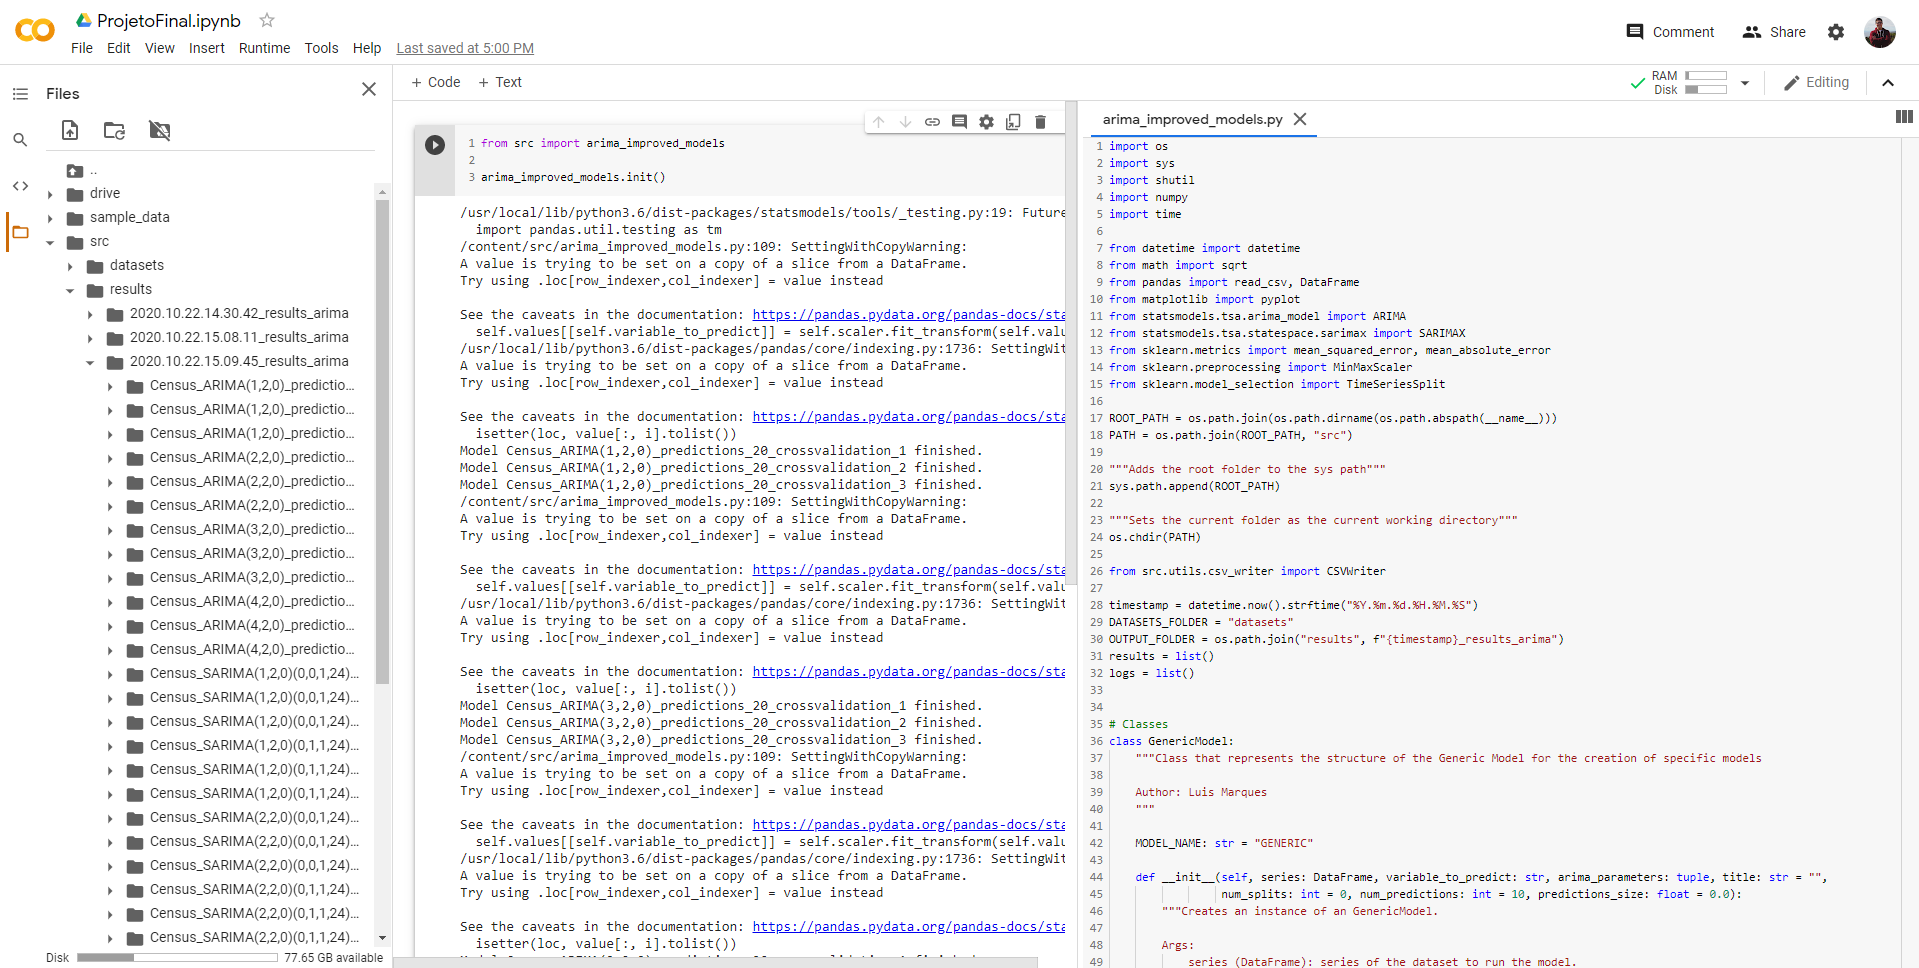
\includegraphics[width=\linewidth]{../private_assets/colab.png}
\caption{Exemplo de um projeto em ambiente de \textit{Google Colab}}
\end{figure}\par

\newpage